% --- Document Class for standard LaTeX (e.g., PDFLaTeX, XeLaTeX, LuaLaTeX) ---
\documentclass{beamer} % English is the default language

% --- Basic Beamer Packages & Settings ---
\usepackage[utf8]{inputenc} % For UTF-8 input encoding (standard for pdfLaTeX)
\usepackage{amsmath}
\usepackage{amssymb}
\usepackage{amsfonts}
\usepackage{bm} % For \bm (bold math)
\usepackage{mathtools} % For \coloneqq, etc.
\usepackage{cases} % For cases environment
\usepackage{graphicx}
\usepackage[svgnames,dvipsnames]{xcolor} % More color names
\usepackage{hyperref}
\hypersetup{
    colorlinks=true,
    linkcolor=NavyBlue,
    citecolor=ForestGreen,
    urlcolor=RoyalBlue,
    pdftitle={Machine Learning Lecture Material},
    pdfauthor={Based on provided materials},
    pdfsubject={Logistic Regression, Gaussian Processes},
    pdfkeywords={Machine Learning, Beamer, LaTeX}
}
\usepackage{cleveref} % Must be loaded after hyperref

% --- Font Settings (from .sty) ---
\usepackage{newpxtext} % For Palatino-like text font
\usepackage{newpxmath} % For math fonts matching newpxtext
\usepackage[T1]{fontenc} % Output T1 encoded fonts for better copy-paste of accented chars

% --- TikZ and tcolorbox (from .sty) ---
\usepackage{tikz}
\usetikzlibrary{shapes.geometric, arrows, positioning, calc, decorations.pathmorphing, fit, backgrounds}
\usepackage{tcolorbox}
\tcbuselibrary{skins,breakable,theorems} % theorems library for \newtcbtheorem

% --- List Customization (from .sty) ---
\usepackage{enumitem}
\setlist[itemize,1]{label=\textbullet}
\setlist[itemize,2]{label=\textendash}
\setlist[itemize,3]{label=$\ast$}
\setlist[enumerate,1]{label=\arabic*.}
\setlist[enumerate,2]{label=\alph*)}
\setlist[enumerate,3]{label=(\roman*)}

% --- Algorithm Packages (from .sty) ---
\usepackage{algorithm}
\usepackage{algpseudocode} % algorithmicx compatible

% --- Listings for code (from .sty) ---
\usepackage{listings}
\lstset{
  basicstyle=\small\ttfamily,
  keywordstyle=\color{blue},
  commentstyle=\color{gray},
  stringstyle=\color{red},
  showstringspaces=false,
  breaklines=true,
  frame=single,
  numbers=left,
  numberstyle=\tiny\color{gray},
  captionpos=b, % caption below
  escapechar=\% % Allows escaping to LaTeX within listings
}

% --- Physics package (from .sty) ---
\usepackage{physics} % For \dd, \pdv, \vb, etc.

% --- Subcaption (from .sty, consider Beamer's columns for side-by-side figures) ---
\usepackage{subcaption}

% --- Custom Math Operators (from .sty and general use) ---
\DeclareMathOperator*{\argmax}{arg\,max}
\DeclareMathOperator*{\argmin}{arg\,min}
\DeclareMathOperator{\diag}{diag}
\DeclareMathOperator{\trace}{Tr} % Trace
\DeclareMathOperator{\rank}{rank} % Rank
\DeclareMathOperator{\Cov}{Cov}   % Covariance
\DeclareMathOperator{\Var}{Var}   % Variance
% \DeclareMathOperator{\E}{\mathbb{E}} % Expectation (already defined by amsmath/amssymb as \mathbb{E})
\newcommand{\E}{\mathbb{E}} % Common shorthand

% --- Custom Commands (from .sty) ---
\newcommand{\mat}[1]{\mathbf{#1}}
\newcommand{\vect}[1]{\mathbf{#1}}
\newcommand{\given}{\,|\,}
\newcommand{\diff}{\mathrm{d}} % For integral dx, etc.

% --- Beamer Theme and Appearance ---
\usetheme{Madrid} % Example theme: Madrid, AnnArbor, Berlin, Singapore, etc.
% \usecolortheme{beaver} % Example color theme

% --- Theorem Environments (adapting .sty to Beamer with tcolorbox - English names) ---
\tcbset{
    theoremstyle/.style={
        enhanced,
        breakable,
        fonttitle=\bfseries,
        coltitle=black,
        separator sign={:\ },
        terminator sign={},
        theorem_separator={ },
        description font=\normalfont,
    }
}

\newtcbtheorem[auto counter, number within=section, crefname={Definition}{Definitions},creflabel={#2#1#3}]{dfn}{Definition}%
{theoremstyle, colback=SkyBlue!10, colframe=SkyBlue!70!Black}{def}

\newtcbtheorem[auto counter, number within=section, crefname={Example}{Examples},creflabel={#2#1#3}]{exm}{Example}%
{theoremstyle, colback=GreenYellow!10, colframe=GreenYellow!60!Black}{ex}

\newtcbtheorem[auto counter, number within=section, crefname={Proposition}{Propositions},creflabel={#2#1#3}]{prop}{Proposition}%
{theoremstyle, colback=Orange!10, colframe=Orange!70!Black}{prop}

\newtcbtheorem[auto counter, number within=section, crefname={Lemma}{Lemmas},creflabel={#2#1#3}]{lem}{Lemma}%
{theoremstyle, colback=Violet!10, colframe=Violet!70!Black}{lem}

\newtcbtheorem[auto counter, number within=section, crefname={Theorem}{Theorems},creflabel={#2#1#3}]{thm}{Theorem}%
{theoremstyle, colback=LightSalmon!20, colframe=LightSalmon!80!Black}{thm}

\newtcbtheorem[auto counter, number within=section, crefname={Corollary}{Corollaries},creflabel={#2#1#3}]{cor}{Corollary}%
{theoremstyle, colback=Gold!10, colframe=Gold!70!Black}{cor}

\newtcbtheorem[auto counter, number within=section, crefname={Remark}{Remarks},creflabel={#2#1#3}]{rem}{Remark}%
{theoremstyle, fonttitle=\bfseries, colback=LightGrey!30, colframe=DarkGrey}{rem}

\newtcbtheorem[auto counter, number within=section, crefname={Exercise}{Exercises},creflabel={#2#1#3}]{exercise}{Exercise}%
{theoremstyle, fonttitle=\bfseries\sffamily, colback=LimeGreen!5, colframe=LimeGreen!50!Black}{exer}


% --- Beamer Settings ---
\beamertemplatenavigationsymbolsempty % Remove navigation symbols if desired
\setbeamertemplate{footline}[frame number] % Show only frame number in footline

% --- Title Information ---
\title{Machine Learning Lecture Material}
\subtitle{Logistic Regression, Gaussian Processes, and Related Mathematical Foundations}
\author{Based on provided materials}
\institute{Your University / Organization Name (Please change accordingly)}
\date{\today}

\begin{document}

% --- Title Page ---
\begin{frame}
  \titlepage
\end{frame}

% --- Table of Contents ---
\begin{frame}{Table of Contents}
  \tableofcontents
\end{frame}

% --- Based on ML2.2.txt content ---
\section{Logistic Regression}
\begin{frame}{Introduction: Review of Logistic Regression}
  \begin{itemize}
    \item The output of linear regression spans all of $\mathbb{R}$.
    \item In classification problems, the target $t \in \{0, 1\}$ (or multiclass).
    \item By passing the output of a linear model $\vect{w}^T \vect{x}$ through a sigmoid function, it can be interpreted as a probability $y \in (0, 1)$.
  \end{itemize}
  \vspace{1em}
  \begin{dfn}[Sigmoid function (Logistic function)]
  \label{def:sigmoid_eng}
  \begin{equation*}
    \sigma(a) = \frac{1}{1 + \exp(-a)}
  \end{equation*}
  \end{dfn}
  Model:
  \begin{equation*}
    y = p(t=1 \given \vect{x}, \vect{w}) = \sigma(\vect{w}^T \vect{x})
  \end{equation*}
\end{frame}

\begin{frame}{Sigmoid Function (Graph)}
  \begin{figure}
    \centering
    \includegraphics[width=0.6\textwidth]{sigmoid_function_image.png}
    \caption{Sigmoid function $\sigma(a) = \frac{1}{1 + \exp(-a)}$ (see \cref{def:sigmoid_eng})}
  \end{figure}
\end{frame}

\begin{frame}{Loss Function: Negative Log-Likelihood}
  For a dataset $\mathcal{D} = \{(\vect{x}_n, t_n)\}_{n=1}^N$, the likelihood function ($t_n \in \{0,1\}$):
  \begin{equation*}
    L(\vect{w}) = p(\vect{t} \given \vect{w}) = \prod_{n=1}^{N} y_n^{t_n} (1 - y_n)^{1 - t_n}
  \end{equation*}
  where $y_n = \sigma(\vect{w}^T \vect{x}_n)$.

  \vspace{1em}
  \begin{dfn}[Negative Log-Likelihood (Cross-Entropy Error Function)]
  \begin{equation*}
    E(\vect{w}) = -\ln L(\vect{w}) = -\sum_{n=1}^{N} \{ t_n \ln y_n + (1 - t_n) \ln(1 - y_n) \}
  \end{equation*}
  \end{dfn}
  The goal is to minimize this.
\end{frame}

\begin{frame}{Gradient}
  The gradient of the error function $E(\vect{w})$ with respect to the parameters $\vect{w}$:
  \begin{equation*}
    \nabla E(\vect{w}) = \sum_{n=1}^{N} (y_n - t_n) \vect{x}_n
  \end{equation*}
  \begin{itemize}
    \item This form is the same as the gradient of the sum-of-squares error in linear regression.
    \item However, $y_n = \sigma(\vect{w}^T \vect{x}_n)$ is non-linear.
    \item Optimization methods like gradient descent are used.
  \end{itemize}
\end{frame}

\begin{frame}{Iteratively Reweighted Least Squares (IRLS)}
  An algorithm to find the maximum likelihood solution $\vect{w}_{\text{ML}}$ for logistic regression.
  \begin{itemize}
    \item There is no analytical solution for $\nabla E(\vect{w}) = \mathbf{0}$.
    \item However, $E(\vect{w})$ is a convex function and has a unique minimum.
    \item Newton-Raphson update rule:
      \begin{equation*}
        \vect{w}_{\text{new}} = \vect{w}_{\text{old}} - \mat{H}^{-1} \nabla E(\vect{w}_{\text{old}})
      \end{equation*}
      where $\mat{H}$ is the Hessian Matrix: $\mat{H} = \nabla \nabla E(\vect{w})$.
  \end{itemize}
\end{frame}

\begin{frame}{Hessian Matrix and IRLS Update Rule}
  The Hessian matrix $\mat{H}$ for the logistic regression error function:
  \begin{equation*}
    \mat{H} = \sum_{n=1}^{N} y_n (1 - y_n) \vect{x}_n \vect{x}_n^T = \mat{X}^T \mat{R} \mat{X}
  \end{equation*}
  Here, $\mat{X}$ is the design matrix (each row is $\vect{x}_n^T$), and $\mat{R}$ is a diagonal matrix with elements $R_{nn} = y_n (1 - y_n)$.

  \vspace{0.5em}
  The Newton-Raphson update rule can be rewritten as (IRLS):
  \begin{equation*}
    \vect{w}_{\text{new}} = (\mat{X}^T \mat{R} \mat{X})^{-1} \mat{X}^T \mat{R} \vect{z}
  \end{equation*}
  This is the form of the normal equations for a weighted least squares problem with weight matrix $\mat{R}$.
  Here, $\vect{z} = \mat{X} \vect{w}_{\text{old}} - \mat{R}^{-1} (\vect{y} - \vect{t})$ is the current "adjusted target".
\end{frame}

\begin{frame}{Multiclass Logistic Regression}
  For $K > 2$ classes: use the Softmax function.
  For activation $a_k = \vect{w}_k^T \vect{x}$, the posterior probability for class $C_k$:
  \begin{equation*}
    y_k(\vect{x}) = p(C_k \given \vect{x}) = \frac{\exp(a_k)}{\sum_{j=1}^{K} \exp(a_j)}
  \end{equation*}
  Loss function (multiclass cross-entropy):
  \begin{equation*}
    E(\vect{w}_1, \dots, \vect{w}_K) = -\sum_{n=1}^{N} \sum_{k=1}^{K} t_{nk} \ln y_{nk}
  \end{equation*}
  $t_{nk}$ is the 1-of-K encoded target.
  \vspace{0.5em}
  Gradient with respect to parameters $\vect{w}_j$:
  \begin{equation*}
    \nabla_{\vect{w}_j} E(\{\vect{w}_k\}) = \sum_{n=1}^{N} (y_{nj} - t_{nj}) \vect{x}_n
  \end{equation*}
  This is similar in form to the two-class case. IRLS can be applied for optimization.
\end{frame}

\section{Gaussian Processes}
\begin{frame}{Introduction: What are Gaussian Processes?}
  \begin{itemize}
    \item A non-parametric Bayesian approach to regression and classification problems.
    \item Performs inference directly in function space, not parameter space.
    \item Basic idea: For any set of input points $\{ \vect{x}_1, \dots, \vect{x}_N \}$, the joint distribution of the function values $\{ f(\vect{x}_1), \dots, f(\vect{x}_N) \}$ follows a multivariate Gaussian distribution.
  \end{itemize}
\end{frame}

\begin{frame}{Definition of a Gaussian Process}
  \begin{dfn}[Gaussian Process (GP)]
  A Gaussian Process (GP) is a collection of random variables, any finite number of which have a joint Gaussian distribution. It is completely specified by:
  \begin{itemize}
    \item \textbf{Mean function} $m(\vect{x})$: $E[f(\vect{x})]$
    \item \textbf{Covariance function (Kernel function)} $k(\vect{x}, \vect{x}')$: $\text{cov}(f(\vect{x}), f(\vect{x}'))$
  \end{itemize}
  A GP is denoted as $f(\vect{x}) \sim \mathcal{GP}(m(\vect{x}), k(\vect{x}, \vect{x}'))$.
  \end{dfn}
  \begin{itemize}
    \item Often, $m(\vect{x}) = 0$ is assumed.
  \end{itemize}
\end{frame}

\begin{frame}{Gaussian Process Regression}
  Given training data $\mathcal{D} = \{(\vect{x}_n, t_n)\}_{n=1}^N$.
  Assume an observation model with noise:
  \begin{equation*}
    t_n = y(\vect{x}_n) + \epsilon_n, \quad \text{where } \epsilon_n \sim \mathcal{N}(0, \beta^{-1})
  \end{equation*}
  $y(\vect{x})$ is a latent function following a GP: $y(\vect{x}) \sim \mathcal{GP}(0, k(\vect{x}, \vect{x}'))$.
  \vspace{0.5em}
  The prior distribution of the target vector $\vect{t} = (t_1, \dots, t_N)^T$ is:
  \begin{equation*}
    p(\vect{t}) = \mathcal{N}(\vect{t} \given \mathbf{0}, \mat{C}_N)
  \end{equation*}
  $\mat{C}_N$ is an $N \times N$ covariance matrix with elements $(C_N)_{nm} = k(\vect{x}_n, \vect{x}_m) + \beta^{-1} \delta_{nm}$.
  $\delta_{nm}$ is the Kronecker delta.
\end{frame}

\begin{frame}{Predictive Distribution}
  We want to find the predictive distribution $p(t_{N+1} \given \vect{t})$ for a new input $\vect{x}_{N+1}$ and its target $t_{N+1}$.
  The joint distribution of $\vect{t}_{N+1} = (t_1, \dots, t_N, t_{N+1})^T = (\vect{t}^T, t_{N+1})^T$ is:
  \begin{equation*}
    p(\vect{t}_{N+1}) = \mathcal{N}(\vect{t}_{N+1} \given \mathbf{0}, \mat{C}_{N+1})
  \end{equation*}
  where $\mat{C}_{N+1}$ is block partitioned as:
  \begin{equation*}
    \mat{C}_{N+1} = \begin{pmatrix} \mat{C}_N & \vect{k} \\ \vect{k}^T & c \end{pmatrix}
  \end{equation*}
  $\vect{k}$ is the vector $(k(\vect{x}_n, \vect{x}_{N+1}))_{n=1}^N$.
  $c = k(\vect{x}_{N+1}, \vect{x}_{N+1}) + \beta^{-1}$.
  \vspace{0.5em}
  From the conditional Gaussian distribution formula, $p(t_{N+1} \given \vect{t}) = \mathcal{N}(t_{N+1} \given m(\vect{x}_{N+1}), \sigma^2(\vect{x}_{N+1}))$:
  \begin{align*}
    \text{Mean: } m(\vect{x}_{N+1}) &= \vect{k}^T \mat{C}_N^{-1} \vect{t} \\
    \text{Variance: } \sigma^2(\vect{x}_{N+1}) &= c - \vect{k}^T \mat{C}_N^{-1} \vect{k}
  \end{align*}
\end{frame}

\begin{frame}{Kernel Function}
  The choice of kernel function $k(\vect{x}, \vect{x}')$ is crucial in determining the properties of the GP.
  \begin{itemize}
    \item Measures similarity between inputs.
    \item Encodes properties like smoothness or periodicity of the function.
  \end{itemize}
  \begin{exm}[Common Kernel Examples]
  \begin{itemize}
    \item \textbf{Linear kernel:} $k(\vect{x}, \vect{x}') = \vect{x}^T \vect{x}'$
    \item \textbf{Polynomial kernel:} $k(\vect{x}, \vect{x}') = (\vect{x}^T \vect{x}' + c)^d$
    \item \textbf{Gaussian kernel (RBF kernel):} $k(\vect{x}, \vect{x}') = \theta_0 \exp\left(-\frac{\theta_1}{2}||\vect{x} - \vect{x}'||^2\right)$
    \item \textbf{Exponential kernel:} $k(\vect{x}, \vect{x}') = \exp\left(-\frac{||\vect{x} - \vect{x}'||}{\ell}\right)$
    \item \textbf{Matérn kernel:} Adjustable smoothness, often more flexible than RBF.
    \item \textbf{Periodic kernel:} Captures periodic patterns.
  \end{itemize}
  \end{exm}
  Kernels have hyperparameters (e.g., $\theta_0, \theta_1$ for RBF, noise precision $\beta$), which are learned, often by maximizing marginal likelihood.
\end{frame}

\begin{frame}{Advantages and Disadvantages of Gaussian Processes}
  \textbf{Advantages:}
  \begin{itemize}
    \item Naturally quantifies uncertainty in predictions (predictive variance).
    \item Flexible modeling through various kernel functions.
    \item Non-parametric; model complexity adapts to data.
    \item Can perform well with relatively small amounts of data.
  \end{itemize}
  \textbf{Disadvantages:}
  \begin{itemize}
    \item Computationally intensive. For $N$ training data points, calculating $\mat{C}_N^{-1}$ is $\mathcal{O}(N^3)$; prediction is $\mathcal{O}(N^2)$.
    \item Difficult to apply to large datasets (requires sparse GP or other approximation methods).
    \item Kernel selection and hyperparameter tuning can be crucial and challenging.
    \item Can have lower interpretability.
  \end{itemize}
\end{frame}

% --- Based on Appendix-ML.txt content ---
\section{Appendix: Mathematical Supplements}
\begin{frame}{Derivative of the Logistic Function}
  The logistic function is $\sigma(x) = \frac{1}{1+e^{-x}}$.
  Its first derivative is:
  \begin{prop}[Derivative of the Logistic Function]
  \begin{align*}
  \frac{\diff\sigma(x)}{\diff x} &= \frac{\diff}{\diff x} (1+e^{-x})^{-1} \\
  &= -1 \cdot (1+e^{-x})^{-2} \cdot \frac{\diff}{\diff x}(1+e^{-x}) \\
  &= - (1+e^{-x})^{-2} \cdot (e^{-x} \cdot (-1)) \\
  &= \frac{e^{-x}}{(1+e^{-x})^2} \\
  \text{Using } \sigma(x) = \frac{1}{1+e^{-x}} \text{ and } 1 - \sigma(x) &= 1 - \frac{1}{1+e^{-x}} = \frac{e^{-x}}{1+e^{-x}}, \text{ we get:}\\
  &= \sigma(x) (1-\sigma(x))
  \end{align*}
  \end{prop}
  This property is important for calculating gradients in logistic regression.
\end{frame}

\begin{frame}{Logistic Function and its Derivative (Graphs)}
  \begin{columns}[T] % T option for top alignment
    \begin{column}{0.5\textwidth}
      \begin{figure}
        \centering
        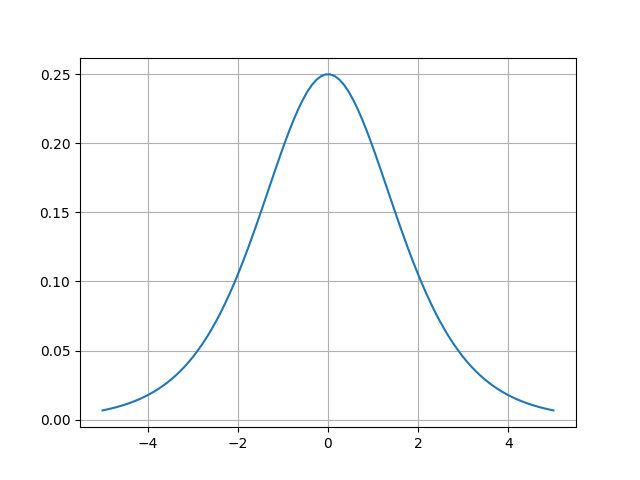
\includegraphics[width=0.9\textwidth]{p1.3.png} % User uploaded p1.1.png
        \caption{Logistic function $\sigma(x)$}
      \end{figure}
    \end{column}
    \begin{column}{0.5\textwidth}
      \begin{figure}
        \centering
        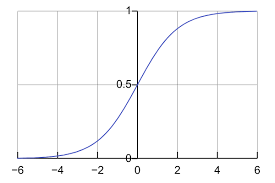
\includegraphics[width=0.9\textwidth]{p1.4.png} % User uploaded p1.2.png
        \caption{Derivative $\sigma(x)(1-\sigma(x))$}
      \end{figure}
    \end{column}
  \end{columns}
\end{frame}

\begin{frame}{Convexity of the Cost Function $J(\theta)$}
  The cost function for logistic regression (negative log-likelihood):
  \begin{equation*}
    J(\theta) = -\frac{1}{m} \sum_{i=1}^m [y^{(i)}\log(h_\theta(x^{(i)})) + (1-y^{(i)})\log(1-h_\theta(x^{(i)}))]
  \end{equation*}
  where $h_\theta(x) = \sigma(\theta^T x)$ is the sigmoid (logistic) function.
  \begin{itemize}
    \item This cost function is convex.
    \item Therefore, optimization algorithms like gradient descent can find the global minimum.
    \item If squared error $(h_\theta(x) - y)^2$ were used for logistic regression, the cost function would be non-convex due to the non-linearity of the sigmoid, potentially having many local minima.
  \end{itemize}
\end{frame}

\begin{frame}{Product of Gaussians}
  The product of two 1D Gaussian distributions is an unnormalized Gaussian distribution.
  \begin{align*}
    \mathcal{N}(x \given \mu_1, \sigma_1^2) &= \frac{1}{\sqrt{2\pi\sigma_1^2}} \exp\left(-\frac{(x-\mu_1)^2}{2\sigma_1^2}\right) \\
    \mathcal{N}(x \given \mu_2, \sigma_2^2) &= \frac{1}{\sqrt{2\pi\sigma_2^2}} \exp\left(-\frac{(x-\mu_2)^2}{2\sigma_2^2}\right)
  \end{align*}
  \begin{prop}[Product of two 1D Gaussians]
  The product $\mathcal{N}(x \given \mu_1, \sigma_1^2) \mathcal{N}(x \given \mu_2, \sigma_2^2) = K \cdot \mathcal{N}(x \given \mu_{\text{new}}, \sigma_{\text{new}}^2)$
  \begin{itemize}
    \item New variance (or precision $1/\sigma^2$):
      \begin{equation*}
        \frac{1}{\sigma_{\text{new}}^2} = \frac{1}{\sigma_1^2} + \frac{1}{\sigma_2^2} \quad \implies \quad \sigma_{\text{new}}^2 = \frac{\sigma_1^2 \sigma_2^2}{\sigma_1^2 + \sigma_2^2}
      \end{equation*}
    \item New mean:
      \begin{equation*}
      \mu_{\text{new}} = \sigma_{\text{new}}^2 \left(\frac{\mu_1}{\sigma_1^2} + \frac{\mu_2}{\sigma_2^2}\right) = \frac{\mu_1\sigma_2^2 + \mu_2\sigma_1^2}{\sigma_1^2 + \sigma_2^2}
      \end{equation*}
  \end{itemize}
  \end{prop}
  $K$ is a normalization constant. This plays a central role in Bayesian updates (e.g., deriving a Gaussian posterior from a Gaussian prior and Gaussian likelihood). A similar form holds for the multivariate case.
\end{frame}

\section{Excerpts and Supplements from PRML}
\begin{frame}{PRML 1.2.3 Bayesian Probabilities}
  \begin{columns}[T]
  \begin{column}{0.5\textwidth}
    \textbf{Frequentist probability:}
    \begin{itemize}
        \item Probability defined as the limit of the frequency of an event in many trials.
        \item Parameters are unknown constants.
    \end{itemize}
  \end{column}
  \begin{column}{0.5\textwidth}
    \textbf{Bayesian probability:}
    \begin{itemize}
        \item Probability interpreted as a degree of uncertainty or belief.
        \item Parameters are also treated as random variables.
    \end{itemize}
  \end{column}
  \end{columns}
  \vspace{1em}
  \begin{thm}[Bayes' Theorem]
  \label{thm:bayes_eng}
  \begin{equation*}
    P(H \given D) = \frac{P(D \given H)P(H)}{P(D)}
  \end{equation*}
  \end{thm}
  \begin{itemize}
    \item $P(H)$: \textbf{Prior} - Belief about hypothesis $H$ before seeing data.
    \item $P(D \given H)$: \textbf{Likelihood} - Probability of observing data $D$ given hypothesis $H$.
    \item $P(H \given D)$: \textbf{Posterior} - Updated belief about hypothesis $H$ after observing data $D$.
    \item $P(D)$: \textbf{Evidence} or Marginal Likelihood. Normalization constant.
      $P(D) = \sum_H P(D \given H)P(H)$ (discrete) or $\int P(D \given H)P(H)dH$ (continuous).
  \end{itemize}
  The Bayesian approach updates beliefs (prior) using observed data (evidence) to obtain a posterior probability.
\end{frame}

\begin{frame}{PRML 1.2.4 The Gaussian Distribution}
  \begin{dfn}[Univariate Gaussian Distribution (Normal Distribution)]
  \begin{equation*}
    \mathcal{N}(x \given \mu, \sigma^2) = \frac{1}{\sqrt{2\pi\sigma^2}} \exp\left( -\frac{1}{2\sigma^2}(x-\mu)^2 \right)
  \end{equation*}
  \end{dfn}
  \begin{itemize}
    \item $\mu$: Mean
    \item $\sigma^2$: Variance
    \item $\beta = 1/\sigma^2$: Precision
  \end{itemize}
  \vspace{0.5em}
  \begin{dfn}[Multivariate Gaussian Distribution for a $D$-dimensional vector $\vect{x}$]
  \begin{equation*}
    \mathcal{N}(\vect{x} \given \boldsymbol{\mu}, \boldsymbol{\Sigma}) = \frac{1}{(2\pi)^{D/2} |\boldsymbol{\Sigma}|^{1/2}} \exp\left( -\frac{1}{2}(\vect{x}-\boldsymbol{\mu})^T \boldsymbol{\Sigma}^{-1} (\vect{x}-\boldsymbol{\mu}) \right)
  \end{equation*}
  \end{dfn}
  \begin{itemize}
    \item $\boldsymbol{\mu}$: $D$-dimensional mean vector
    \item $\boldsymbol{\Sigma}$: $D \times D$ covariance matrix
  \end{itemize}
  The Gaussian distribution is widely used in statistics and machine learning due to its analytical tractability and its ability to approximate many real-world phenomena via the Central Limit Theorem.
\end{frame}

\begin{frame}{PRML 1.5 Decision Theory}
  Decision theory provides a mathematical framework for making optimal decisions under uncertainty, combined with probability theory.
  \begin{block}{Regression Problems}
    \begin{itemize}
      \item Objective: Determine a function $y(\vect{x})$ to predict a target $t$ for an input $\vect{x}$.
      \item Define a loss function $L(t, y(\vect{x}))$ (e.g., squared loss $L(t, y(\vect{x})) = (y(\vect{x}) - t)^2$).
      \item Goal is to minimize the expected loss:
        \begin{equation*}
          \mathbb{E}[L] = \iint L(t, y(\vect{x})) p(\vect{x}, t) d\vect{x} dt
        \end{equation*}
      \item For squared loss, the $y(\vect{x})$ that minimizes expected loss is the conditional expectation $\mathbb{E}[t \given \vect{x}]$:
        \begin{equation*}
         y(\vect{x}) = \int t p(t \given \vect{x}) dt
        \end{equation*}
    \end{itemize}
  \end{block}
\end{frame}

\begin{frame}{PRML 1.5 Decision Theory (Continued)}
  \begin{block}{Classification Problems}
  \begin{itemize}
    \item Objective: Assign an input $\vect{x}$ to one of $K$ classes $C_k$.
    \item Loss matrix $L_{kj}$: Loss incurred for misclassifying a sample whose true class is $C_k$ as class $C_j$.
    \item Goal is to minimize expected loss. Often, this means minimizing the misclassification rate.
      This is equivalent to choosing the class with the maximum posterior probability $p(C_k \given \vect{x})$.
    \item \textbf{Reject option:} Choice to refuse prediction if the model's prediction is uncertain (e.g., if the maximum posterior probability is below some threshold).
  \end{itemize}
  \end{block}
  \vspace{0.5em}
  General stages of decision theory:
  \begin{enumerate}
      \item Inference stage: Learn or compute necessary probability distributions, like $p(\vect{x},t)$ or $p(C_k \given \vect{x})$.
      \item Decision stage: Use these probabilities to make optimal decisions.
  \end{enumerate}
\end{frame}

\begin{frame}{PRML 2.1.1 Binary Variables and the Beta Distribution}
  A single binary random variable $x \in \{0, 1\}$ (e.g., heads $x=1$ in a coin toss).
  \begin{dfn}[Bernoulli Distribution]
  \begin{equation*}
    \text{Bern}(x \given \mu) = \mu^x (1-\mu)^{1-x}
  \end{equation*}
  \end{dfn}
  Here $P(x=1) = \mu$. $\mathbb{E}[x] = \mu$, $\text{var}(x) = \mu(1-\mu)$.
  \vspace{0.5em}
  The number of times $x=1$ occurs in $N$ independent trials, $m$, follows the \textbf{Binomial Distribution}:
  \begin{dfn}[Binomial Distribution]
  \begin{equation*}
    \text{Bin}(m \given N,\mu) = \binom{N}{m} \mu^m (1-\mu)^{N-m}
  \end{equation*}
  \end{dfn}
  $\mathbb{E}[m] = N\mu$, $\text{var}(m) = N\mu(1-\mu)$.
  \vspace{0.5em}
  \begin{dfn}[Beta Distribution] A conjugate prior for the parameter $\mu \in [0,1]$.
  \begin{equation*}
    \text{Beta}(\mu \given a,b) = \frac{\Gamma(a+b)}{\Gamma(a)\Gamma(b)} \mu^{a-1} (1-\mu)^{b-1}
  \end{equation*}
  \end{dfn}
  $\mathbb{E}[\mu] = \frac{a}{a+b}$. $a, b$ are hyperparameters, interpretable as effective observation counts.
  After observing a dataset $\mathcal{D}$ ($m$ occurrences of $x=1$, $l$ occurrences of $x=0$, $N=m+l$), the posterior is $\text{Beta}(\mu \given m+a, l+b)$.
\end{frame}

\begin{frame}{PRML 2.3.6 Bayesian Linear Regression}
  For a linear regression model $y(\vect{x}, \vect{w}) = \vect{w}^T \boldsymbol{\phi}(\vect{x})$, introduce a prior distribution for parameters $\vect{w}$.
  Prior distribution: $p(\vect{w}) = \mathcal{N}(\vect{w} \given \vect{m}_0, \mat{S}_0)$ (often, $\vect{m}_0=\mathbf{0}, \mat{S}_0=\alpha^{-1}\mat{I}$ is assumed).
  Likelihood function: $p(\vect{t} \given \vect{w}) = \mathcal{N}(\vect{t} \given \mat{\Phi}\vect{w}, \beta^{-1}\mat{I})$. ($\beta$ is noise precision)
  \vspace{0.5em}
  The posterior distribution $p(\vect{w} \given \vect{t}) \propto p(\vect{t} \given \vect{w}) p(\vect{w})$ is also Gaussian.
  $p(\vect{w} \given \vect{t}) = \mathcal{N}(\vect{w} \given \vect{m}_N, \mat{S}_N)$
  where,
  \begin{align*}
    \mat{S}_N &= (\mat{S}_0^{-1} + \beta \mat{\Phi}^T \mat{\Phi})^{-1} \\
    \vect{m}_N &= \mat{S}_N (\mat{S}_0^{-1} \vect{m}_0 + \beta \mat{\Phi}^T \vect{t})
  \end{align*}
  For a simple prior ($\vect{m}_0=\mathbf{0}, \mat{S}_0=\alpha^{-1}\mat{I}$):
  \begin{align*}
    \vect{m}_N &= \beta \mat{S}_N \mat{\Phi}^T \vect{t} \\
    \mat{S}_N &= (\alpha\mat{I} + \beta \mat{\Phi}^T \mat{\Phi})^{-1}
  \end{align*}
  The posterior mean $\vect{m}_N$ coincides with the MAP (Maximum A Posteriori) estimate.
\end{frame}

\begin{frame}{PRML 2.3.6 Predictive Distribution in Bayesian LR}
  The predictive distribution for a new input $\vect{x}^*$ and target $t^*$, $p(t^* \given \vect{x}^*, \vect{t}, \alpha, \beta)$, is obtained by integrating (marginalizing) $p(t^* \given \vect{w}, \beta)$ over the posterior distribution of $\vect{w}$.
  \begin{equation*}
    p(t^* \given \vect{x}^*, \vect{t}, \alpha, \beta) = \int p(t^* \given \vect{w}, \beta) p(\vect{w} \given \vect{t}) d\vect{w}
  \end{equation*}
  This results in a Gaussian distribution:
  \begin{equation*}
    p(t^* \given \vect{x}^*, \vect{t}, \alpha, \beta) = \mathcal{N}(t^* \given \vect{m}_N^T \boldsymbol{\phi}(\vect{x}^*), \sigma_N^2(\vect{x}^*))
  \end{equation*}
  where the predictive variance $\sigma_N^2(\vect{x}^*)$ is:
  \begin{equation*}
    \sigma_N^2(\vect{x}^*) = \frac{1}{\beta} + \boldsymbol{\phi}(\vect{x}^*)^T \mat{S}_N \boldsymbol{\phi}(\vect{x}^*)
  \end{equation*}
  \begin{itemize}
    \item The first term ($1/\beta$): Inherent noise in the data.
    \item The second term ($\boldsymbol{\phi}(\vect{x}^*)^T \mat{S}_N \boldsymbol{\phi}(\vect{x}^*)$): Due to uncertainty in parameters $\vect{w}$. As more training data is available, $\mat{S}_N$ becomes smaller, and this term also decreases.
  \end{itemize}
\end{frame}


\begin{frame}[allowframebreaks]{References}
  \begin{thebibliography}{9}
    \bibitem{Bishop2006}
    Bishop, C. M. (2006). \textit{Pattern Recognition and Machine Learning}. Springer.
    \bibitem{YourLectureNotesEng}
    (Your lecture note title, etc., please add as appropriate)
  \end{thebibliography}
\end{frame}

\end{document}